\documentclass[tikz,border=8pt]{standalone}
\usepackage{amsmath,amssymb}
\usepackage{tikz}
\usetikzlibrary{arrows.meta,calc,decorations.pathreplacing,patterns,shapes.geometric,positioning,shadings}

\begin{document}
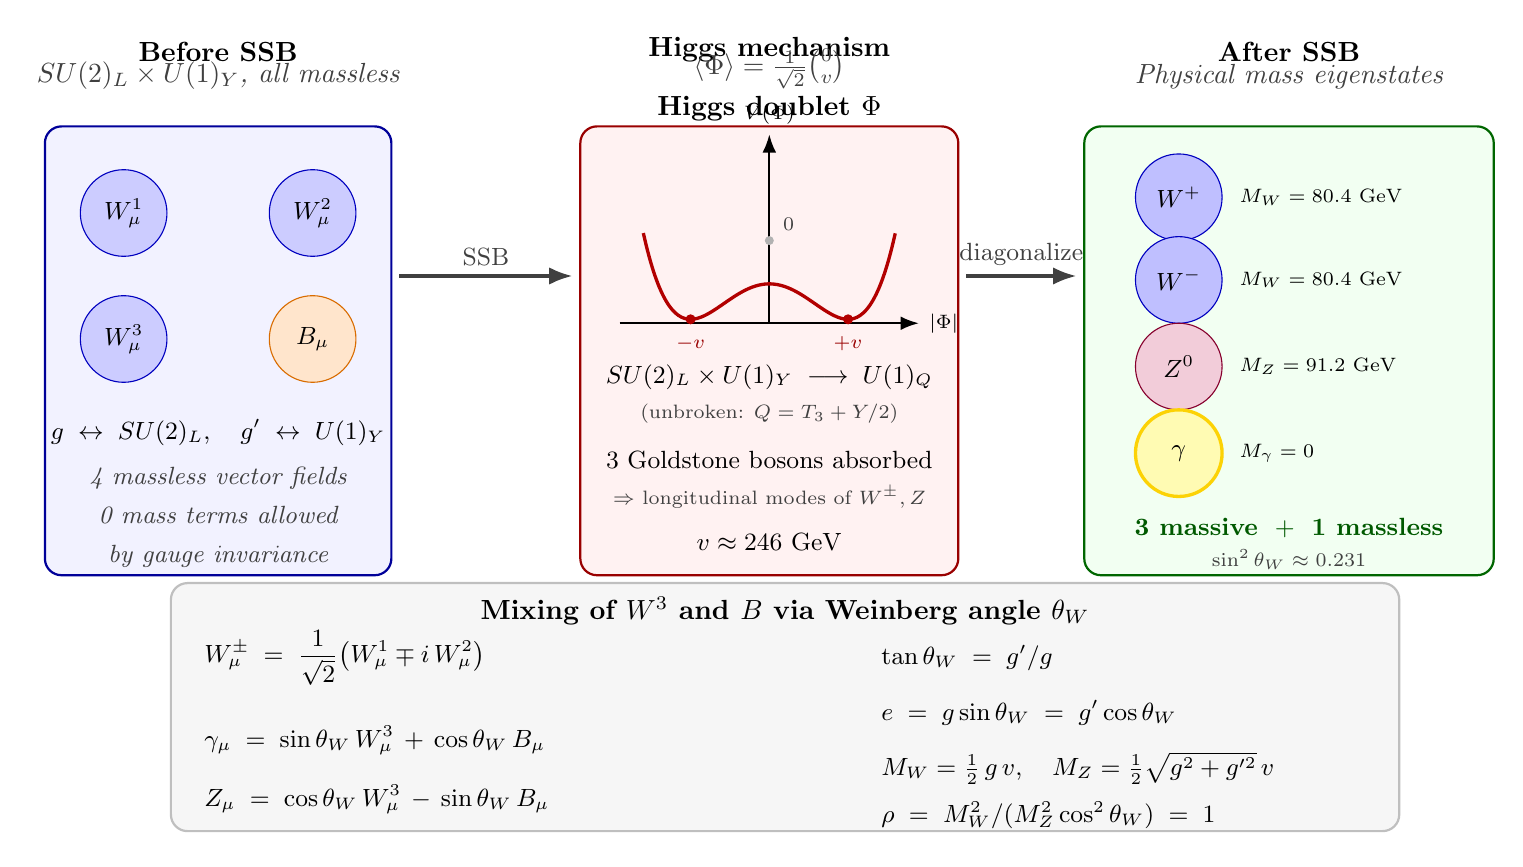
\begin{tikzpicture}[>=Latex, font=\small]

% =====================================================================
% Electroweak symmetry breaking diagram
% Left:  4 massless gauge bosons W^1, W^2, W^3, B  under SU(2)_L x U(1)_Y
% Middle: Higgs SSB step (Mexican-hat icon, vacuum value v)
% Right: physical states W^+, W^- (massive), Z (massive), gamma (massless)
%        plus Weinberg-angle mixing relations
% =====================================================================

% --------- Left column: unbroken gauge bosons ----------------------------
\def\Lx{-7.0}     % left column x
\def\Mx{0.0}      % middle column x (Higgs)
\def\Rx{6.6}      % right column x

% Title bars
\node[anchor=south, font=\bfseries]
  at (\Lx,3.6) {Before SSB};
\node[anchor=south, font=\itshape, text=gray!50!black]
  at (\Lx,3.25) {$SU(2)_L \times U(1)_Y$, all massless};

\node[anchor=south, font=\bfseries]
  at (\Mx,3.6) {Higgs mechanism};
\node[anchor=south, font=\itshape, text=gray!50!black]
  at (\Mx,3.25) {$\langle\Phi\rangle = \tfrac{1}{\sqrt 2}\binom{0}{v}$};

\node[anchor=south, font=\bfseries]
  at (\Rx,3.6) {After SSB};
\node[anchor=south, font=\itshape, text=gray!50!black]
  at (\Rx,3.25) {Physical mass eigenstates};

% Box around left column
\draw[rounded corners=6pt, thick, blue!60!black, fill=blue!5]
  (\Lx-2.2,-2.8) rectangle (\Lx+2.2,2.9);

% Four massless gauge boson nodes on the left
\def\rW{0.55}

% W^1
\filldraw[blue!75!black, fill=blue!20]
  (\Lx-1.2, 1.8) circle (\rW);
\node at (\Lx-1.2, 1.8) {$W^{1}_\mu$};

% W^2
\filldraw[blue!75!black, fill=blue!20]
  (\Lx+1.2, 1.8) circle (\rW);
\node at (\Lx+1.2, 1.8) {$W^{2}_\mu$};

% W^3
\filldraw[blue!75!black, fill=blue!20]
  (\Lx-1.2, 0.2) circle (\rW);
\node at (\Lx-1.2, 0.2) {$W^{3}_\mu$};

% B
\filldraw[orange!85!black, fill=orange!20]
  (\Lx+1.2, 0.2) circle (\rW);
\node at (\Lx+1.2, 0.2) {$B_\mu$};

% Couplings label
\node[anchor=north, font=\small]
  at (\Lx, -0.7)
  {$g \;\leftrightarrow\; SU(2)_L,\quad g' \;\leftrightarrow\; U(1)_Y$};

\node[anchor=north, font=\small\itshape, text=gray!50!black]
  at (\Lx, -1.3) {4 massless vector fields};
\node[anchor=north, font=\small\itshape, text=gray!50!black]
  at (\Lx, -1.8) {0 mass terms allowed};
\node[anchor=north, font=\small\itshape, text=gray!50!black]
  at (\Lx, -2.3) {by gauge invariance};

% --------- Middle column: Higgs Mexican hat ----------------------------
\draw[rounded corners=6pt, thick, red!60!black, fill=red!5]
  (\Mx-2.4,-2.8) rectangle (\Mx+2.4,2.9);

% Mexican-hat potential sketch (cross-section)
% Plot V(phi) = -mu^2 phi^2 + lambda phi^4 schematic
\def\hatY{1.4}    % vertical center of hat plot

% Axes
\draw[->, thick] (\Mx-1.9,\hatY-1.0) -- (\Mx+1.9,\hatY-1.0)
  node[right, font=\scriptsize] {$|\Phi|$};
\draw[->, thick] (\Mx,\hatY-1.0) -- (\Mx,\hatY+1.4)
  node[above, font=\scriptsize] {$V(\Phi)$};

% Mexican-hat curve (symmetric double well in cross section)
\draw[very thick, red!70!black]
  plot[domain=-1.6:1.6, samples=80, smooth]
  ({\Mx + \x},{\hatY-1.0 + 0.45*(\x*\x - 1.0)*(\x*\x - 1.0) + 0.05});

% Mark vacuum point at +v
\filldraw[red!70!black] (\Mx+1.0,\hatY-0.95) circle (1.6pt);
\node[anchor=north, font=\scriptsize, text=red!60!black]
  at (\Mx+1.0,\hatY-1.05) {$+v$};
\filldraw[red!70!black] (\Mx-1.0,\hatY-0.95) circle (1.6pt);
\node[anchor=north, font=\scriptsize, text=red!60!black]
  at (\Mx-1.0,\hatY-1.05) {$-v$};

% Origin marker
\filldraw[gray!60] (\Mx,\hatY+0.05) circle (1.4pt);
\node[anchor=south west, font=\scriptsize, text=gray!50!black]
  at (\Mx+0.05,\hatY+0.05) {$0$};

% Higgs label
\node[anchor=south, font=\bfseries]
  at (\Mx, \hatY+1.45) {Higgs doublet $\Phi$};

% Below the hat: SSB explanation
\node[anchor=north, font=\small]
  at (\Mx, -0.0)
  {$SU(2)_L \times U(1)_Y \;\longrightarrow\; U(1)_Q$};
\node[anchor=north, font=\scriptsize, text=gray!50!black]
  at (\Mx, -0.5) {(unbroken: $Q = T_3 + Y/2$)};

\node[anchor=north, font=\small]
  at (\Mx, -1.1)
  {3 Goldstone bosons absorbed};
\node[anchor=north, font=\scriptsize, text=gray!50!black]
  at (\Mx, -1.55)
  {$\Rightarrow$ longitudinal modes of $W^\pm, Z$};

\node[anchor=north, font=\small]
  at (\Mx, -2.15)
  {$v \approx 246~\mathrm{GeV}$};

% --------- Right column: physical mass eigenstates ----------------------
\draw[rounded corners=6pt, thick, green!40!black, fill=green!5]
  (\Rx-2.6,-2.8) rectangle (\Rx+2.6,2.9);

% W^+
\filldraw[blue!75!black, fill=blue!25]
  (\Rx-1.4, 2.0) circle (\rW);
\node at (\Rx-1.4, 2.0) {$W^{+}$};
\node[anchor=west, font=\scriptsize]
  at (\Rx-0.75, 2.0) {$M_W = 80.4~\mathrm{GeV}$};

% W^-
\filldraw[blue!75!black, fill=blue!25]
  (\Rx-1.4, 0.95) circle (\rW);
\node at (\Rx-1.4, 0.95) {$W^{-}$};
\node[anchor=west, font=\scriptsize]
  at (\Rx-0.75, 0.95) {$M_W = 80.4~\mathrm{GeV}$};

% Z
\filldraw[purple!70!black, fill=purple!20]
  (\Rx-1.4,-0.15) circle (\rW);
\node at (\Rx-1.4,-0.15) {$Z^{0}$};
\node[anchor=west, font=\scriptsize]
  at (\Rx-0.75,-0.15) {$M_Z = 91.2~\mathrm{GeV}$};

% gamma (photon, massless)
\filldraw[yellow!70!orange, fill=yellow!30, very thick]
  (\Rx-1.4,-1.25) circle (\rW);
\node at (\Rx-1.4,-1.25) {$\gamma$};
\node[anchor=west, font=\scriptsize]
  at (\Rx-0.75,-1.25) {$M_\gamma = 0$};

% Massive vs massless tag
\node[anchor=north, font=\small\bfseries, text=green!35!black]
  at (\Rx,-1.95) {3 massive $\;+\;$ 1 massless};
\node[anchor=north, font=\scriptsize, text=gray!50!black]
  at (\Rx,-2.35) {$\sin^2\theta_W \approx 0.231$};

% --------- Arrows: left to middle, middle to right ---------------------
\draw[->, very thick, gray!50!black]
  (\Lx+2.3,1.0) -- (\Mx-2.5,1.0)
  node[midway, above, font=\small] {SSB};
\draw[->, very thick, gray!50!black]
  (\Mx+2.5,1.0) -- (\Rx-2.7,1.0)
  node[midway, above, font=\small] {diagonalize};

% --------- Mixing relations panel (below the row) -----------------------
\def\PY{-4.4}      % panel y center
\draw[rounded corners=6pt, thick, gray!50, fill=gray!7]
  (-7.6,\PY-1.65) rectangle (8.0,\PY+1.5);

\node[anchor=north, font=\bfseries]
  at (0.2,\PY+1.45) {Mixing of $W^{3}$ and $B$ via Weinberg angle $\theta_W$};

% Charged combinations
\node[anchor=west, font=\small] at (-7.3,\PY+0.55)
  {$W^{\pm}_\mu \;=\; \dfrac{1}{\sqrt 2}\bigl(W^{1}_\mu \mp i\,W^{2}_\mu\bigr)$};

% Photon and Z mixing
\node[anchor=west, font=\small] at (-7.3,\PY-0.5)
  {$\gamma_\mu \;=\; \sin\theta_W\, W^{3}_\mu \,+\, \cos\theta_W\, B_\mu$};

\node[anchor=west, font=\small] at (-7.3,\PY-1.25)
  {$Z_\mu \;=\; \cos\theta_W\, W^{3}_\mu \,-\, \sin\theta_W\, B_\mu$};

% Right block: relations
\node[anchor=west, font=\small] at (1.3,\PY+0.55)
  {$\tan\theta_W \;=\; g'/g$};

\node[anchor=west, font=\small] at (1.3,\PY-0.15)
  {$e \;=\; g\sin\theta_W \;=\; g'\cos\theta_W$};

\node[anchor=west, font=\small] at (1.3,\PY-0.85)
  {$M_W = \tfrac{1}{2}\,g\,v,\quad M_Z = \tfrac{1}{2}\sqrt{g^2+g'^2}\,v$};

\node[anchor=west, font=\small] at (1.3,\PY-1.45)
  {$\rho \;=\; M_W^2/(M_Z^2\cos^2\theta_W) \;=\; 1$};

\end{tikzpicture}
\end{document}
